\begin{table*}[t]
\centering
\caption{Mean net bits and median DRD on all-method matched images.}
\label{tab:multiload}
\begin{tabular*}{\textwidth}{@{\extracolsep{\fill}}rrcccccccc@{}}
\toprule
& & \multicolumn{2}{c}{\textbf{Proposed ABM}} &
\multicolumn{2}{c}{\textbf{Dong}} &
\multicolumn{2}{c}{\textbf{Huynh--Nguyen}} &
\multicolumn{2}{c}{\textbf{PPOCP}} \\
\cmidrule(lr){3-4}\cmidrule(lr){5-6}\cmidrule(lr){7-8}\cmidrule(lr){9-10}
\textbf{Target} & \textbf{Matched} & \textbf{Net} & \textbf{DRD} &
\textbf{Net} & \textbf{DRD} & \textbf{Net} & \textbf{DRD} &
\textbf{Net} & \textbf{DRD} \\
\midrule
64  & 86 & $-57$ & 0.041 & $-224$ & 0.056 & $-2200$ & 0.035 & $-997$ & 0.023 \\
128 & 83 & $-7$  & 0.080 & $-176$ & 0.108 & $-2096$ & 0.070 & $-1653$ & 0.041 \\
256 & 69 & \textbf{93} & 0.135 & $-81$ & 0.200 & $-1812$ & 0.117 & $-2856$ & 0.064 \\
512 & 46 & \textbf{309} & 0.176 & 96 & 0.332 & $-1191$ & 0.178 & $-4822$ & 0.097 \\
\bottomrule
\end{tabular*}
\end{table*}

\begin{table*}[t]
\centering
\caption{Fixed-cohort sensitivity analysis on the 46 images available for
every method and payload. Values are mean net bits with 95\% bootstrap
intervals; DRD is the cohort median.}
\label{tab:fixed-cohort}
\resizebox{\textwidth}{!}{
\begin{tabular}{@{}rccc@{}}
\toprule
\textbf{Target} & \textbf{Method} & \textbf{Mean net bits (95\% CI)} &
\textbf{Median DRD}\\
\midrule
64 & Proposed ABM & $-48.5\;[-49.0,-48.0]$ & 0.022\\
   & Dong / Huynh--Nguyen / PPOCP & $-226.3\;[-229.6,-223.0]$ /
   $-1644.7\;[-1854.3,-1447.5]$ / $-1028.0\;[-1063.3,-990.1]$ &
   0.029 / 0.024 / 0.012\\
128 & Proposed ABM & $8.0\;[5.7,10.1]$ & 0.043\\
   & Dong / Huynh--Nguyen / PPOCP & $-178.3\;[-187.8,-169.9]$ /
   $-1582.8\;[-1792.4,-1386.8]$ / $-1707.8\;[-1767.5,-1643.0]$ &
   0.066 / 0.044 / 0.025\\
256 & Proposed ABM & $113.9\;[108.3,119.0]$ & 0.087\\
   & Dong / Huynh--Nguyen / PPOCP & $-83.8\;[-105.6,-65.7]$ /
   $-1456.3\;[-1656.2,-1260.9]$ / $-2954.1\;[-3060.2,-2835.8]$ &
   0.132 / 0.084 / 0.050\\
512 & Proposed ABM & $309.0\;[289.7,325.9]$ & 0.176\\
   & Dong / Huynh--Nguyen / PPOCP & $95.8\;[55.1,131.0]$ /
   $-1190.6\;[-1397.6,-996.7]$ / $-4821.7\;[-5025.6,-4607.1]$ &
   0.332 / 0.178 / 0.097\\
\bottomrule
\end{tabular}}
\end{table*}

Table~\ref{tab:fixed-cohort} preserves the ordering observed in the
\RevisionAddBegin
payload-specific matched analysis. It also shows that ABM reaches a positive
128-bit mean on the fixed cohort.
\RevisionAddEnd

\begin{figure*}[t]
\centering
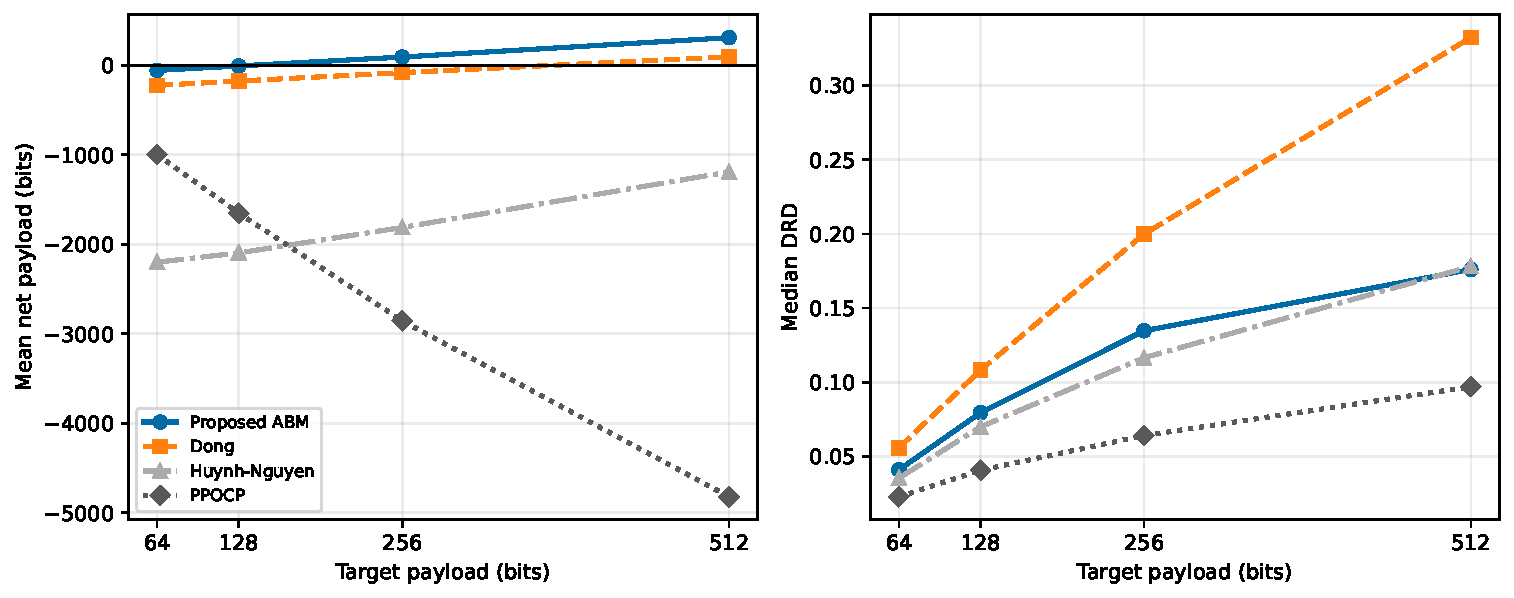
\includegraphics[width=\textwidth]{images/Figure_5.pdf}
\caption{Payload scaling on all-method matched images: mean net payload
(left) and median DRD (right), with 95\% bootstrap confidence bands.}
\label{fig:multiload}
\end{figure*}

Figure~\ref{fig:protocol-overview} complements the table with availability and
\RevisionAddBegin
the net-bits--DRD operating curves. PPOCP carries every target on all
\RevisionAddEnd
test images. ABM availability progresses from 89\% at 64 bits to 70\% at 512
bits, matching Dong at the highest target and remaining above Huynh--Nguyen.
\RevisionAddBegin
The right panel is descriptive because the methods span different DRD ranges;
Table~\ref{tab:fixed-cohort} provides the
\RevisionAddEnd
controlled cross-payload comparison.

\begin{figure*}[t]
\centering
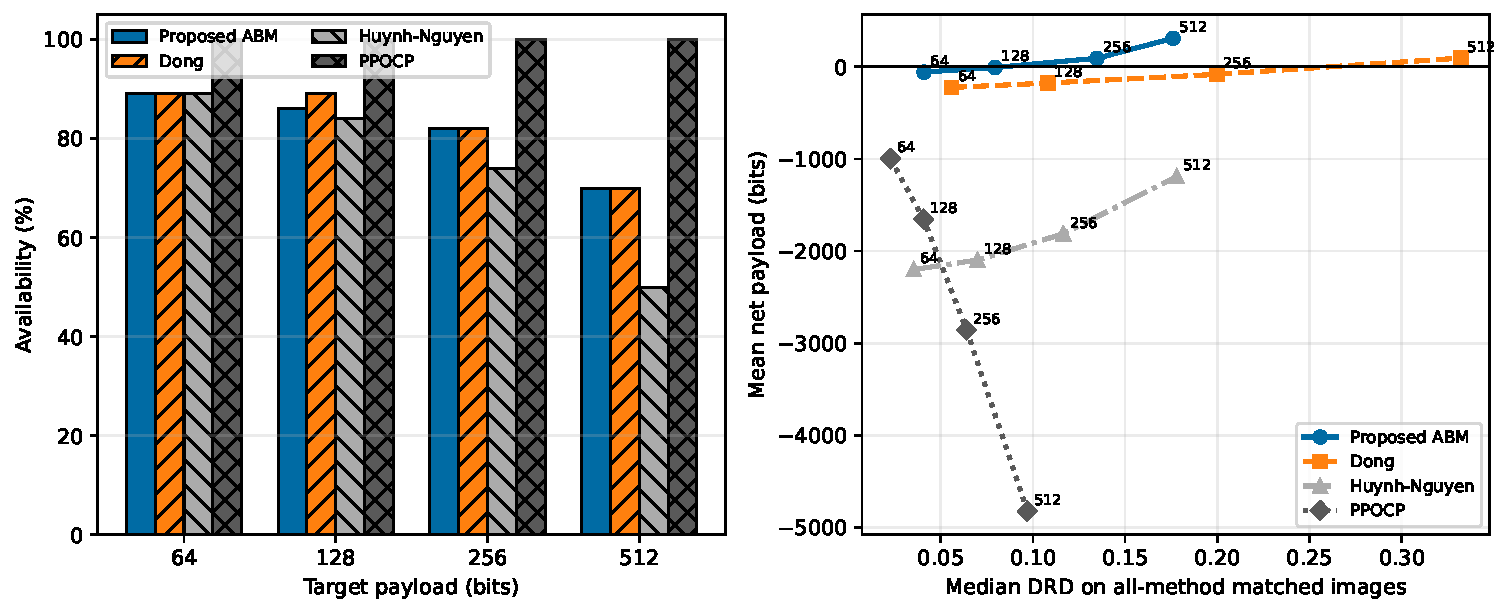
\includegraphics[width=\textwidth]{images/Figure_6.pdf}
\caption{Complementary views of payload feasibility and useful-capacity
efficiency. Error bars denote 95\% bootstrap confidence intervals for mean net
payload; numbers on the right panel denote target payloads in bits.}
\label{fig:protocol-overview}
\end{figure*}

\subsection{Paired Significance and Binarization Strata}

At each payload, ABM's paired net advantage over Dong, Huynh--Nguyen, and
PPOCP remains significant after Holm correction. At 256 bits, adjusted
$p$-values are below $6.7\times10^{-13}$, $3.1\times10^{-13}$, and
$2.2\times10^{-14}$, respectively. Median ABM net gains are 160, 1752, and
\RevisionAddBegin
3016 bits, with paired rank-biserial correlations of 0.974, 1.000, and 1.000.
DRD tests place ABM below Dong and above the perceptually focused PPOCP and
Huynh--Nguyen curves, yielding a two-objective interpretation.
\RevisionAddEnd

Binarization suitability is defined before embedding: threshold 128 must agree
with Otsu on at least 95\% of pixels, and foreground fraction must lie in
$[0.05,0.95]$. Twenty-two test images satisfy this criterion. As shown in
Figure~\ref{fig:binarization}, ABM is available on all 22 through 256 bits,
while net-positive behavior at 256 and 512 bits is present in both strata.
\RevisionAddBegin
Suitability therefore serves as an applicability indicator, with net
performance reported separately in both strata.
\RevisionAddEnd

At 512 bits, the 70 available images have mean foreground fraction 0.289,
189.2 eligible non-uniform PEAK patterns, and non-uniform $8\times8$ block
fraction 0.227. The 30 unavailable images have corresponding means 0.025,
\RevisionAddBegin
34.2, and 0.024. Unavailable cases are therefore concentrated in near-empty or
nearly uniform thresholded photographs with too few repeated non-uniform
patterns; available cases still restore the message and cover exactly.
\RevisionAddEnd

\begin{figure*}[t]
\centering
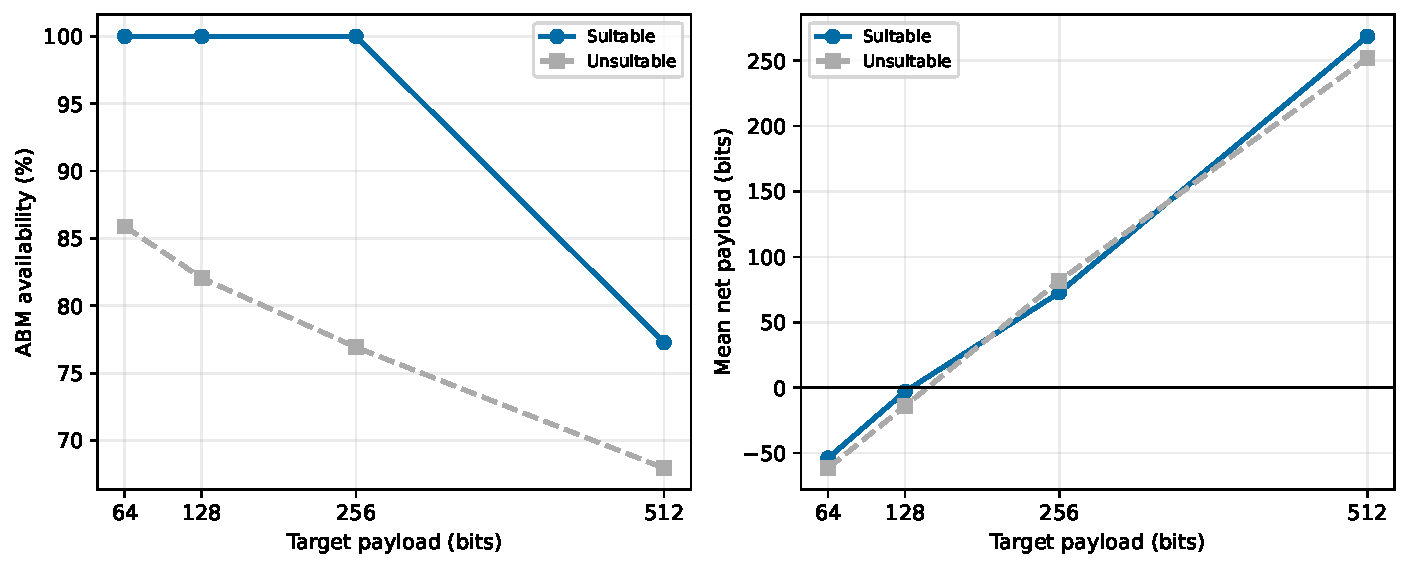
\includegraphics[width=0.92\textwidth]{images/Figure_7.pdf}
\caption{ABM availability and mean net payload after stratification by
fixed-threshold/Otsu agreement.}
\label{fig:binarization}
\end{figure*}

\subsection{Runtime and Memory}

Figure~\ref{fig:resources} and Table~\ref{tab:resources} report the 256-bit
resource benchmark on ten protocol images. PPOCP provides the shortest runtime,
Huynh--Nguyen the smallest incremental memory profile, and ABM requires a
median runtime of 3.56 s and median incremental peak RSS of 2.56 MiB.
Dong's complete ten-divisor optimization
quantifies the computational cost of per-image context search.

\begin{table*}[t]
\centering
\caption{Median resource profile at a 256-bit target.}
\label{tab:resources}
\begin{tabular}{@{}lrrr@{}}
\toprule
\textbf{Method} & \textbf{Available} & \textbf{Time (s)} &
\textbf{Peak RSS increase (MiB)} \\
\midrule
Proposed ABM & 9/10 & 3.56 & 2.56 \\
Dong & 9/10 & 16.97 & 0.05 \\
Huynh--Nguyen & 7/10 & 1.51 & 0.02 \\
PPOCP & 10/10 & 0.16 & 0.70 \\
\bottomrule
\end{tabular}
\end{table*}

Table~\ref{tab:abm-module-runtime} decomposes the proposed method on the eight
document images at the 75\% payload budget. Candidate generation, including
CNN-ranked distance-one assignment, and embedding dominate runtime; the
enumerative serialization itself is negligible.

\begin{table}[t]
\centering
\caption{ABM runtime decomposition by module on document images.}
\label{tab:abm-module-runtime}
\begin{tabular}{@{}lr@{}}
\toprule
\textbf{Module} & \textbf{Median time (s)} \\
\midrule
Candidate generation and ranking & 0.5771 \\
Serialized-prefix optimization & 0.2832 \\
Embedding & 0.7155 \\
Serialization & 0.00015 \\
Extraction & 0.1926 \\
Round-trip verification & 0.00008 \\
\midrule
End-to-end total & 1.7857 \\
\bottomrule
\end{tabular}
\vspace{2pt}
{\footnotesize\RaggedRight The end-to-end timer includes minor orchestration
overhead outside the module timers.\par}
\end{table}

\begin{figure*}[t]
\centering
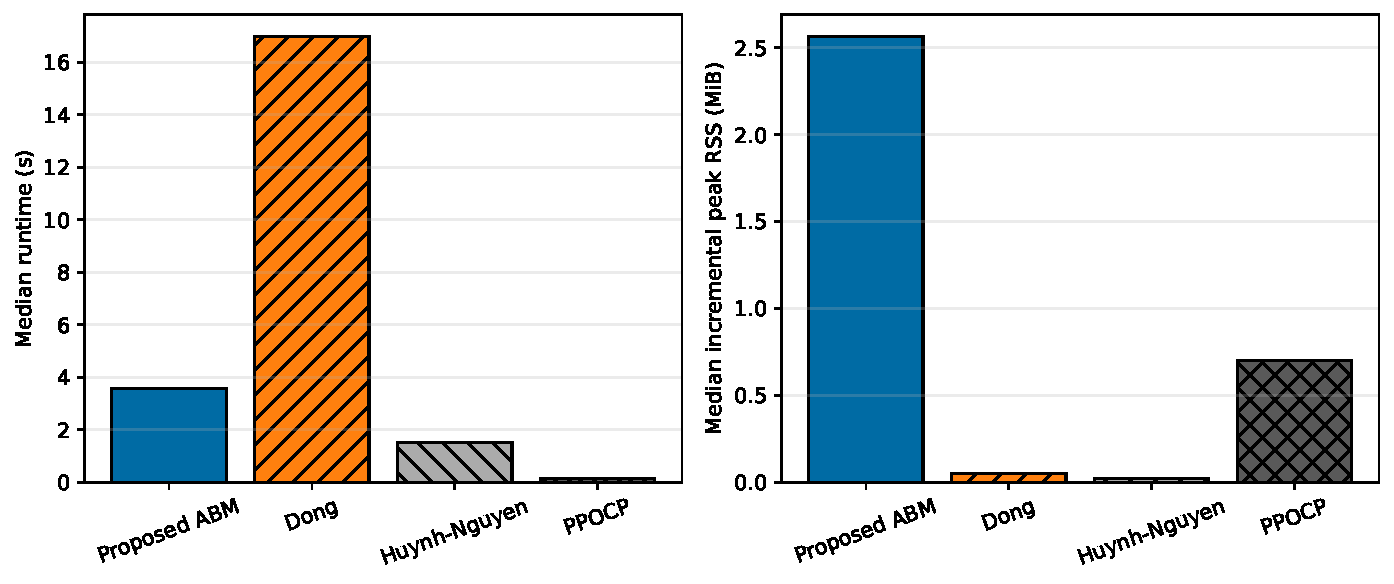
\includegraphics[width=0.92\textwidth]{images/Figure_8.pdf}
\caption{Median wall-clock runtime and incremental peak RSS at 256 bits.}
\label{fig:resources}
\end{figure*}

\subsection{Grouped Steganalysis}
\label{subsec:steganalysis}

The security evaluation uses foreground fraction, horizontal and vertical
transition rates, and normalized $2\times2$ and $3\times3$ pattern histograms.
Five-fold GroupKFold keeps each cover and its stego in the same fold. Both a
standardized logistic model and a 500-tree Random Forest are evaluated.

Figure~\ref{fig:steganalysis} visualizes the complete AUC curves, and
Table~\ref{tab:steganalysis} reports the logistic detector. PPOCP provides the
\RevisionAddBegin
most resistant curve from 128 to 512 bits. ABM's AUC increases with useful
payload, making statistical footprint the principal signal for future
optimization. The Random Forest gives ABM AUC values 0.623, 0.691,
\RevisionAddEnd
0.769, and 0.851, confirming the same payload trend with a different model.
\RevisionAddBegin

A document-image payload sweep explains this trend. When the ABM payload
fraction increases from 25\% to 100\%, mean net payload rises from 329 to 3203
bits, but the mean Jensen--Shannon divergence between cover and marked
$3\times3$ pattern histograms also rises from 0.0087 to 0.0409. Mean
horizontal and vertical transition-rate displacements rise from
0.0032/0.0032 to 0.0127/0.0128. The steganalysis features therefore respond to
the same PEAK/ZERO redistribution that produces useful capacity: repeated PEAK
patterns are depleted and distance-one ZERO patterns are populated. High
payload is therefore best interpreted as capacity-oriented reversible
annotation in access-controlled channels. Figure~\ref{fig:visual-comparison}
gives the qualitative counterpart: residual locations show how each method
distributes its changes under the same 512-bit target on table1-3.
\RevisionAddEnd

\begin{table*}[t]
\centering
\caption{Grouped logistic-detector ROC AUC on matched cover/stego pairs.}
\label{tab:steganalysis}
\begin{tabular}{@{}rccccc@{}}
\toprule
\textbf{Target} & \textbf{Pairs} & \textbf{Proposed ABM} &
\textbf{Dong} & \textbf{Huynh--Nguyen} & \textbf{PPOCP} \\
\midrule
64  & 86 & 0.706 & 0.656 & \textbf{0.599} & 0.653 \\
128 & 83 & 0.826 & 0.759 & 0.688 & \textbf{0.654} \\
256 & 69 & 0.900 & 0.784 & 0.774 & \textbf{0.691} \\
512 & 46 & 0.957 & 0.896 & 0.909 & \textbf{0.690} \\
\bottomrule
\end{tabular}
\end{table*}

\begin{figure*}[t]
\centering
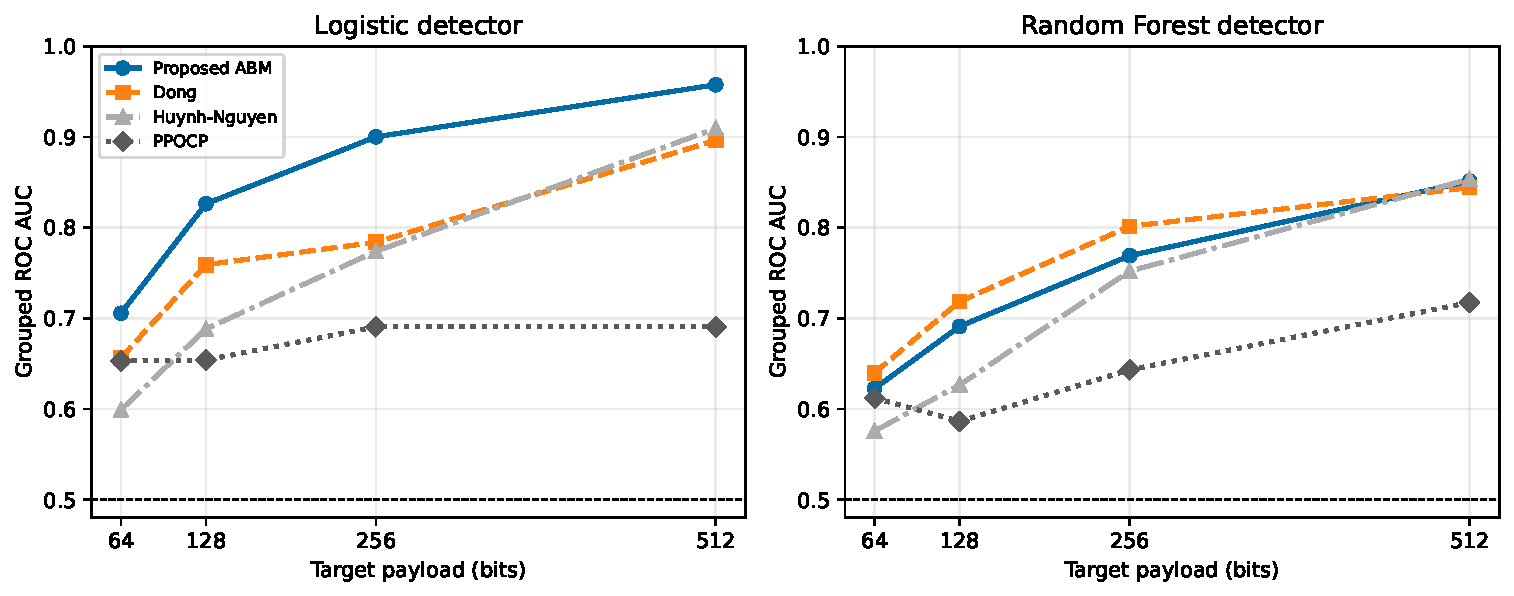
\includegraphics[width=\textwidth]{images/Figure_9.pdf}
\caption{Grouped steganalysis across payloads with logistic (left) and Random
Forest (right) detectors. The dashed line denotes chance-level AUC.}
\label{fig:steganalysis}
\end{figure*}

\begin{figure*}[t]
\centering
\begin{minipage}{0.49\textwidth}
\centering
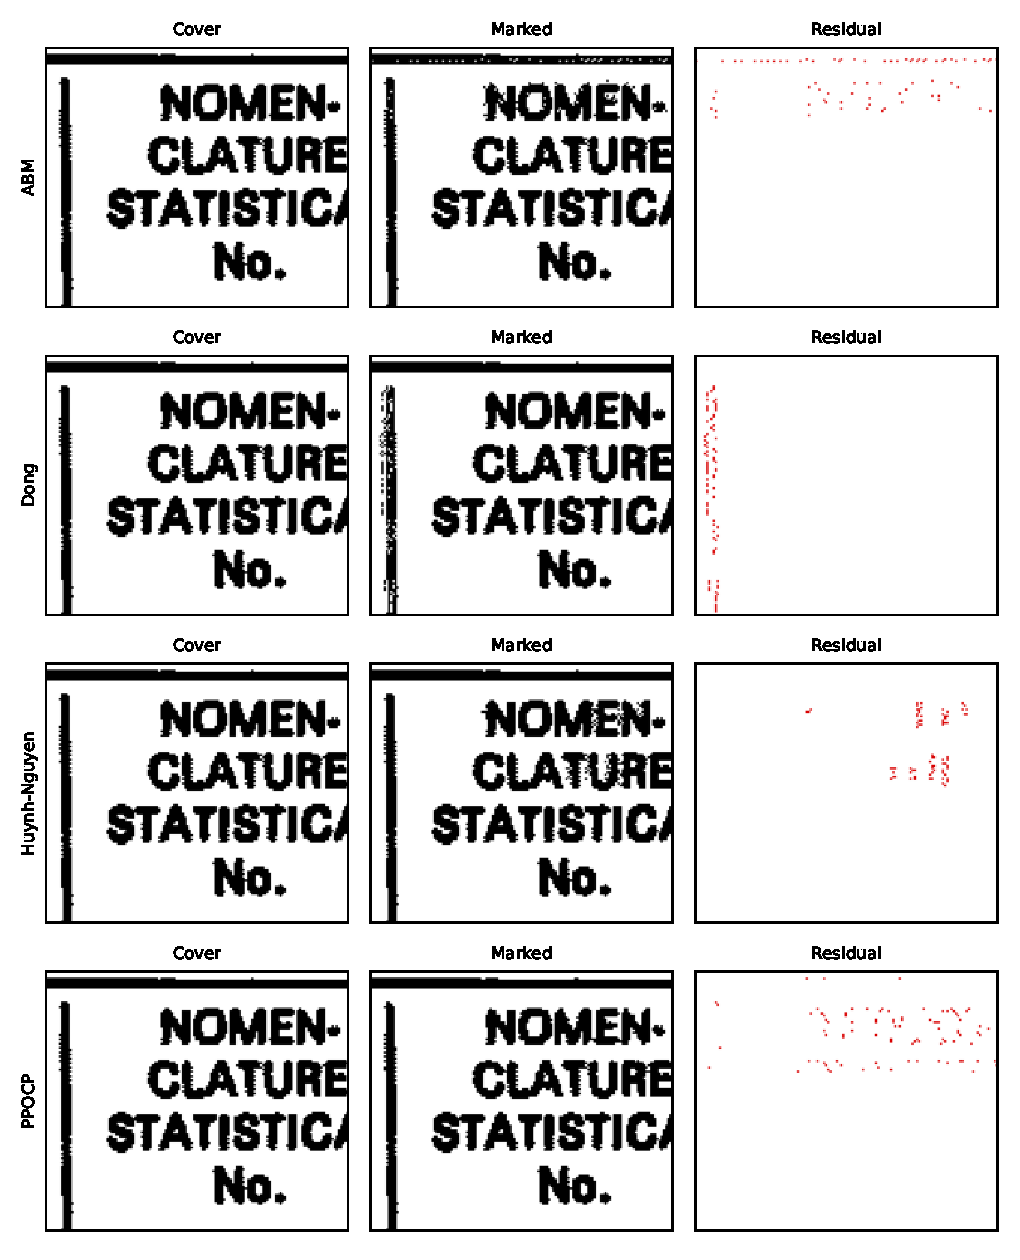
\includegraphics[width=\linewidth,trim=0 300bp 0 0,clip]{images/Figure_10.pdf}
\end{minipage}\hfill
\begin{minipage}{0.49\textwidth}
\centering
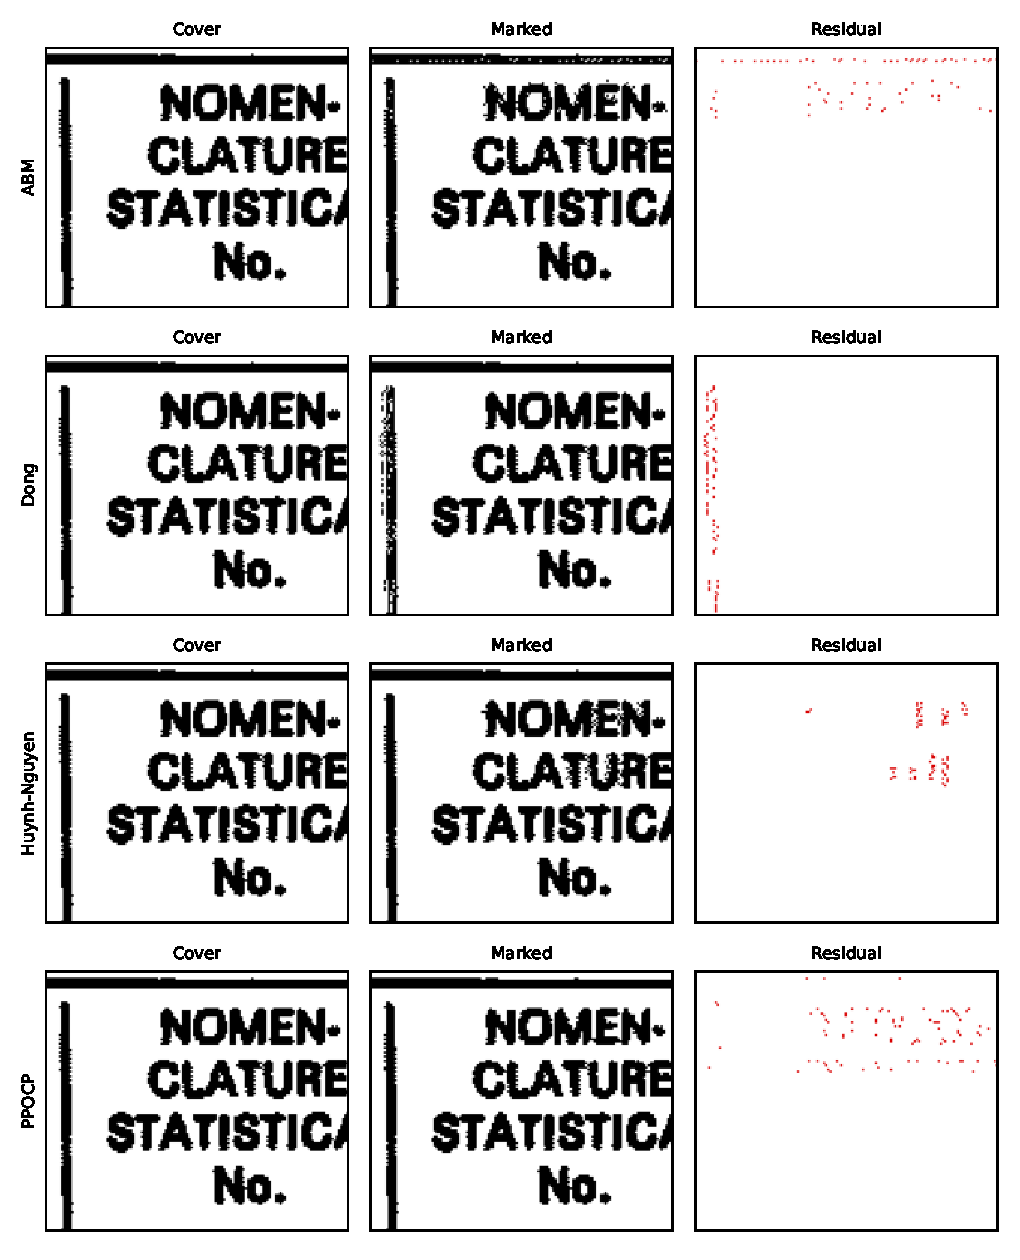
\includegraphics[width=\linewidth,trim=0 0 0 325bp,clip]{images/Figure_10.pdf}
\end{minipage}
\caption{Cover, marked, and residual zooms on table1-3 at a 512-bit target,
split into two panels to fit the two-column layout: ABM and Dong appear on the left, and
Huynh--Nguyen and PPOCP on the right. Residual pixels are
shown in red on the marked crop to make modification locations visible under
the same payload.}
\label{fig:visual-comparison}
\end{figure*}

\section{Discussion}
\label{sec:discussion}

\subsection{Positioning Across Practical Objectives}

\RevisionAddBegin
The experiments separate four objectives that are frequently merged in RDH
comparisons. In the BOSSbase common protocol, ABM provides the highest
net-payload curve and crosses into mean-positive net payload between 128 and
256 bits on the payload-specific matched cohorts. In perceptual quality, PPOCP
defines the lowest median DRD, followed closely by Huynh--Nguyen at the higher
target. In applicability, PPOCP has universal target availability, while ABM
combines high availability with compact side information. In computational
cost, ABM remains practical and is substantially faster than the complete Dong
parameter search.
\RevisionAddEnd

This decomposition supports a specific, protocol-bounded position: among the
four evaluated implementations, ABM provides the highest net payload after
serialized metadata, whereas PPOCP provides the lowest-distortion and
\RevisionAddBegin
most favorable detectability profile. This conclusion rests on exact round trips,
\RevisionAddEnd
multi-payload curves, a fixed-cohort sensitivity analysis, and paired tests.
Because synchronization formats materially affect net payload, the result is
\RevisionAddBegin
framed as a protocol-bounded comparison of the evaluated implementations.
\RevisionAddEnd

\RevisionAddBegin
FUNSD separates external-document transfer from net efficiency. The frozen
codec remains exactly reversible on every available run and A2 reduces
auxiliary cost on every paired operating point under both binarizations, which
materially strengthens the evidence for transfer of the reversible mechanism
and the serialization-aware activation rule. At the same time, mean delivered
net payload remains negative through 512 bits and positive-net cases are rare.
Those values characterize the tested low-to-moderate-payload operating regime
on scanned documents; they should not be generalized into a claim of positive
net efficiency on FUNSD.
\RevisionAddEnd

\subsection{Security-Aware Optimization Direction}

\RevisionAddBegin
The measured AUC curves and content-adaptive detectability principles
\cite{Sedighi2018Content} suggest a direct route for strengthening the method.
The current CNN predicts reciprocal-distance cost, whereas the steganalysis
\RevisionAddEnd
features respond to shifts in local pattern distributions. A security-aware
ranker can optimize
\begin{equation}
\mathcal{L}(Z_j)=
\beta\,\widehat{\mathrm{DRD}}(Z_j)
+\gamma\,\Delta_{\mathrm{hist}}(Z_j)
+\eta\,\Delta_{\mathrm{trans}}(Z_j),
\label{eq:security-aware-ranker}
\end{equation}
where $\Delta_{\mathrm{hist}}$ measures the change in local pattern histograms
and $\Delta_{\mathrm{trans}}$ measures transition-rate displacement. The
coefficients can be selected on a Pareto front of net bits, DRD, and grouped
detector AUC. This extension builds directly on the validated ranker and
preserves the exact reversible wire format.

